\documentclass[pdflatex,compress]{beamer}

%\usetheme[dark,framenumber,totalframenumber]{ElektroITK}
\usetheme[darktitle,framenumber,totalframenumber]{ElektroITK}

\renewcommand{\figurename}{Gambar} \setbeamertemplate{caption}[numbered]

\usepackage{graphicx}
\usepackage{multicol}

\title{FORENSIKA SUARA}
\subtitle{Konsep Dasar Sinyal dan Sistem Audio}

\author{Tim Dosen Pengampu}

\begin{document}

\maketitle

\section{Pendahuluan}

\begin{frame}
	\frametitle{Pendahuluan}
	\begin{itemize}
		\item Ilmu akustik dan audio engineering merupakan dasar dari audio forensik.
		\item Bukti audio forensik meliputi audio recording. \item Representasi dari bunyi yang dideteksi di udara oleh mikrofon, dikonversi menjadi tegangan, dan kemudian disimpan dalam suatu media.
		\item Rekaman audio bisa berupa analog maupun digital.
		\item Studi tentang akustik melibatkan prinsip fisika dari propagasi bunyi di udara.
	\end{itemize}
\end{frame}

\begin{frame}
	\frametitle{Pendahuluan}
	\begin{itemize}
		\item Untuk memahami dan menginterpretasikan rekaman forensik, perlu memahami konsep akustik sehingga bunyi yang dideteksi di dalam rekaman dapat dianalisis dan dikaitkan dengan karakteristik pemantulan (reflection), penyerapan (absorption), difraksi (diffraction), dan gema/dengung (reverberation) dari bunyi.
	\end{itemize}
\end{frame}

\section{Bunyi}

\begin{frame}
	\frametitle{Bunyi}
	\begin{itemize}
		\item Bunyi di udara merupakan hasil dari getaran.
		\item Permukaan yang bergetar menyebabkan partikel-partikel bergerak maju mundur dalam jarak pendek.
		\item Permukaan bergerak ke depan $\rightarrow$ partikel udara di dekat permukaan didorong (compressed), permukaan bergerak mundur $\rightarrow$ partikel udara di dekat permukaan ditarik (expanded/rarified).
		\item Partikel udara yang mengalami compressed-expanded tadi akan melakukan hal yang sama terhadap partikel udara di dekatnya, dan seterusnya.
		\item Menghasilkan gelombang yang menjauhi permukaan yang bergetar.
	\end{itemize}
\end{frame}

\begin{frame}
	\frametitle{Gerakan partikel udara}
	\begin{figure}
		\centering
		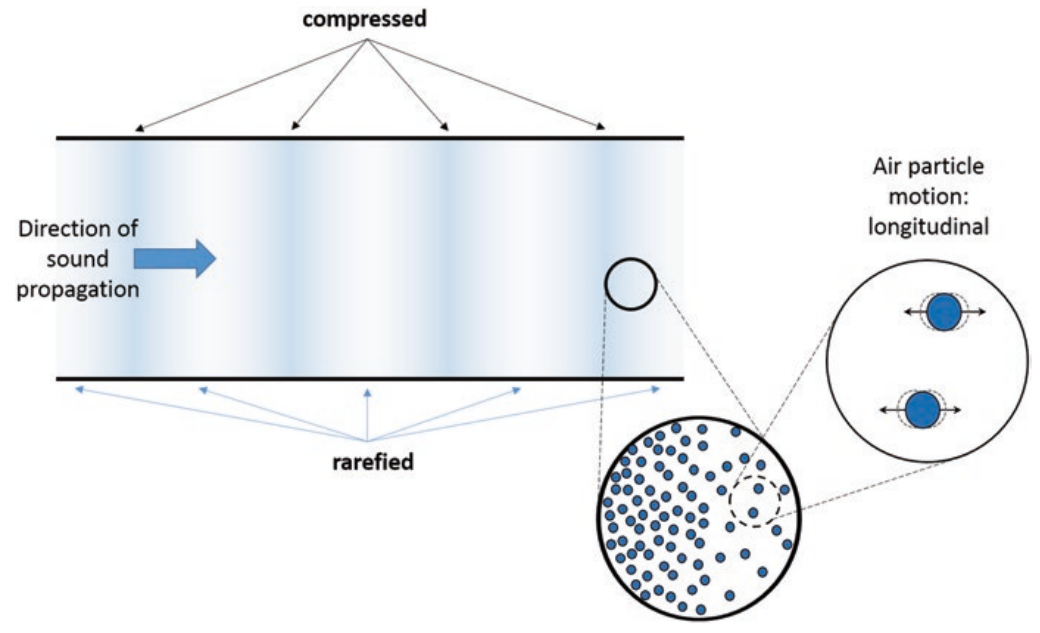
\includegraphics[width=0.7\linewidth]{img/img001}
		\caption[]{Gerakan partikel udara di dalam gelombang bunyi: longitudinal (maju dan mundur) sejajar dengan arah propagasi.}
		\label{fig:img001}
	\end{figure}
\end{frame}

\begin{frame}
	\frametitle{Tekanan akustik}
	\begin{itemize}
		\item Gelombang bunyi adalah gelombang longitudinal.
		\item Karena gerakan longitudinal sulit untuk digambarkan, maka penggambarannya berdasarkan tekanan akustik terhadap waktu.
		\item Tekanan akustik sangat kecil jika dibandingkan dengan tekanan atmosfir normal.
		\item Tekanan di atas permukaan laut $ \approx 1 \times 10^5 $ Pa.
		\item Suara terkecil yang dapat didengar memiliki tekanan sebesar $ 2 \times 10^{-5} $ Pa.
		\item Suara yang sangat keras (konser atau mesin di industri) $\approx$ 1 Pa.
	\end{itemize}
\end{frame}

\section{Tingkat Tekanan Bunyi}

\begin{frame}
	\frametitle{Tingkat Tekanan Bunyi}
	\begin{itemize}
		\item Sound pressure level (SPL) / tingkat tekanan bunyi.
		\item Tekanan akustik yang dapat didengar berada di rentang $ 2 \times 10^{-5} $ hingga 1 Pa.
		\item Rentang yang dapat didengar diubah ke dalam satuan logaritmik agar bunyi yang paling senyap berada pada level zero dan yang paling keras berada di dalam 2 atau 3 angka saja.
		\[ B = \log_{10}\frac{(\text{daya}_1)}{(\text{daya}_0)} \] atau 
		\[ B = \log_{10}\frac{(\text{intensitas}_1)}{(\text{intensitas}_0)} \]
		\item B adalah bel, daya dalam Watt dan intensitas dalam W/m$ ^2 $
	\end{itemize}
\end{frame}

\begin{frame}
	\frametitle{Tingkat Tekanan Bunyi}
	\begin{itemize}
		\item Agar dapat menggunakan definisi bel di atas untuk bunyi, perlu dilakukan konversi dari tekanan akustik (pascal) ke intensitas akustik (W/m$ ^2 $).
		\item Hubungan antara gelombang bunyi adalah intensitas akustik proporsional dengan kuadrat dari tekanan akustik, sehingga
		\[ B = \log_{10}\frac{(\text{tekanan}_1^2)}{(\text{tekanan}_0^2)} = 2\log_{10}\frac{(\text{tekanan}_1)}{(\text{tekanan}_0)} \]
		\item decibel [dB] = presisi 1/10 dari bel.
		\[ \text{decibel}[dB] = 20 \log_{10} \frac{tekanan_1}{tekanan_0}  \]
	\end{itemize}
\end{frame}

\begin{frame}
	\frametitle{Tingkat Tekanan Bunyi}
	\begin{itemize}
		\item SPL dalam decibel $\rightarrow \text{tekanan}_0 = 20~ \mu\text{Pa}$ dan $ \text{tekanan}_1 $ = tekanan efektif atau RMS yang diukur di mikrofon.
		\item Dipilih 20 $\mu$Pa karena batas dari pendengaran manusia.
		\item Jika ada sinyal akustik dengan tekanan efektif sebesar 20 $\mu$Pa, maka SPL nya adalah 0 dB.
		\item Gelombang bunyi yang berpropagasi di udara memiliki kecepatan bunyi sebesar 343 m/s dalam suhu ruang 20$^\circ$C.
	\end{itemize}
\end{frame}

\section{Panjang Gelombang, Frekuensi dan Spektrum}
\begin{frame}
	\frametitle{Panjang Gelombang dan Frekuensi}
	\begin{itemize}
		\item Jika sumber suara berosilasi, bunyi akan memiliki siklus tekanan tinggi dan rendah.
		\item Waktu yang dibutuhkan dalam satu kali osilasi disebut periode getaran.
		\item Selama waktu yang dibutuhkan dalam 1 kali osilasi, tekanan bunyi akan berpropagasi di udara sejauh jarak tertentu. Jarak ini disebut panjang gelombang.
		\item Osilasi bunyi diekspresikan dalam laju osilasi, yaitu berapa banyak siklus osilasi dalam 1 detik.
		\item Laju osilasi ini yang disebut dengan frekuensi.
	\end{itemize}
\end{frame}

\begin{frame}
	\frametitle{Panjang Gelombang dan Frekuensi}
	\begin{itemize}
		\item Jika osilasinya sedikit (frekuensinya rendah), periode dari tiap siklus akan berdurasi tinggi, sehingga gelombang akan berpropagasi lebih jauh dalam satu siklus.
		\item Frekuensi lebih rendah $\rightarrow$ panjang gelombang lebih panjang.
		\item Begitu juga sebaliknya.
		\item Hubungan antara frekuensi $ f $ dan panjang gelombang $ \lambda $ adalah $ c = f\lambda $, dimana $ c $ adalah kecepatan bunyi (m/s).
	\end{itemize}
\end{frame}

\begin{frame}
	\frametitle{Panjang Gelombang dan Frekuensi}
	\begin{figure}
		\centering
		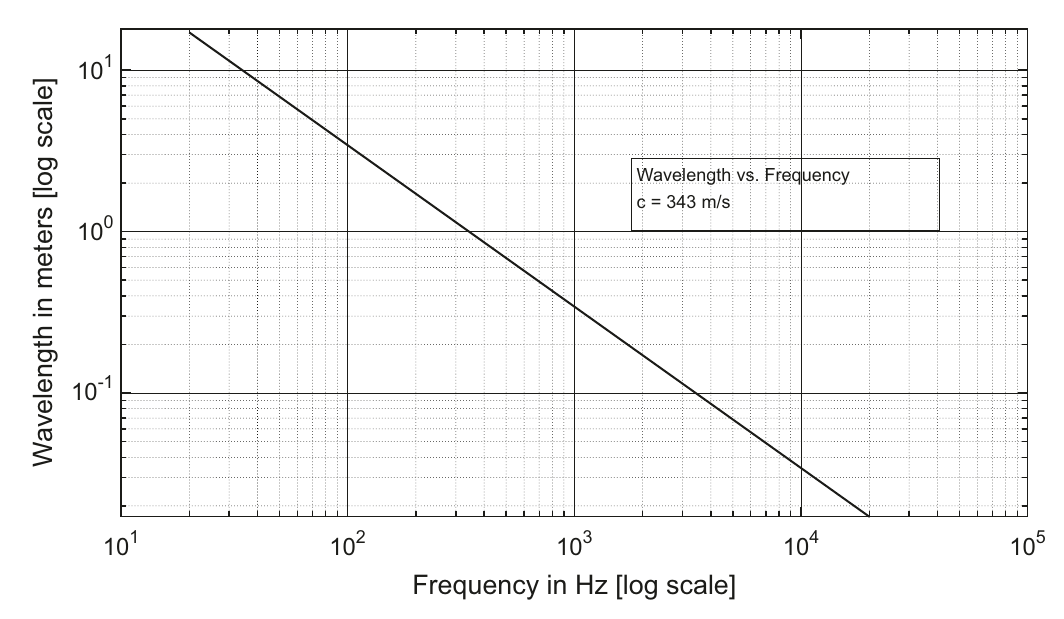
\includegraphics[width=0.9\linewidth]{img/img002}
		\caption{Perkalian antara frekuensi terhadap panjang gelombang adalah kecepatan bunyi.}
		\label{fig:img002}
	\end{figure}
\end{frame}

\begin{frame}
	\frametitle{Sinewave}
	\begin{itemize}
		\item Jenis paling sederhana dari bunyi yang memiliki energi pada frekuensi tunggal adalah pure tone.
		\item Bentuk gelombang (waveform) dari bunyi frekuensi tunggal ini seperti pada Gambar \ref{fig:img003}.
		\item Disebut juga sinewave atau sinusoidal.
		\item Sumbu y dapat berupa tekanan, tegangan, atau perpindahan (displacement) dan sumbu x adalah waktu.
		\item Gambar \ref{fig:img003} memiliki T = 1 md dan frekuensi = 1/T = 1 kHz.
		\item Untuk sinewave dengan interval yang lebih lama ditunjukkan oleh Gambar \ref{fig:img004}.
	\end{itemize}
\end{frame}

\begin{frame}
	\frametitle{Sinewave}
	\begin{figure}
		\centering
		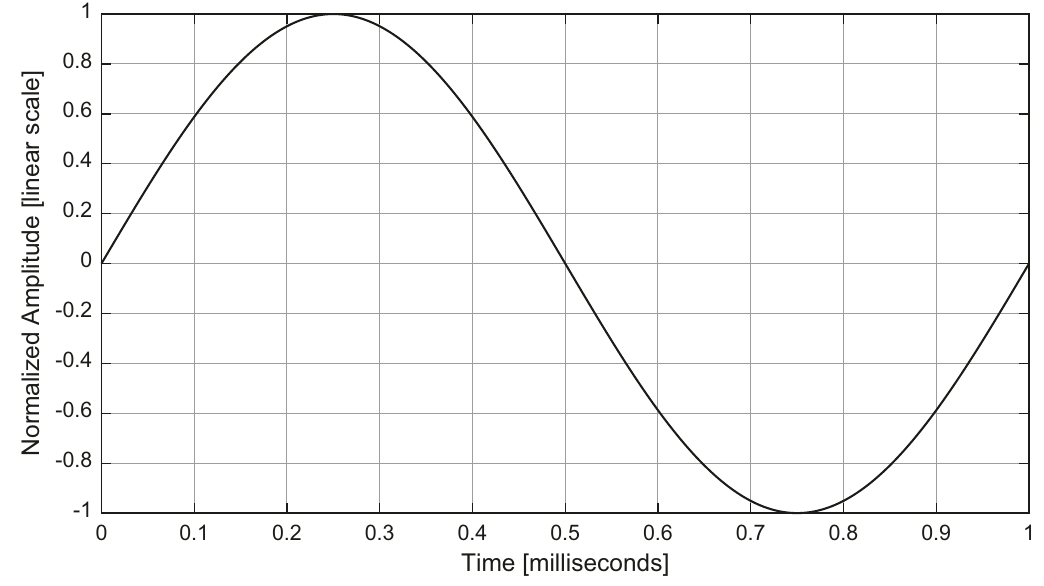
\includegraphics[width=0.7\linewidth]{img/img003}
		\caption{Sinewave 1 kHz}
		\label{fig:img003}
	\end{figure}
\end{frame}

\begin{frame}
	\frametitle{Sinewave}
	\begin{figure}
		\centering
		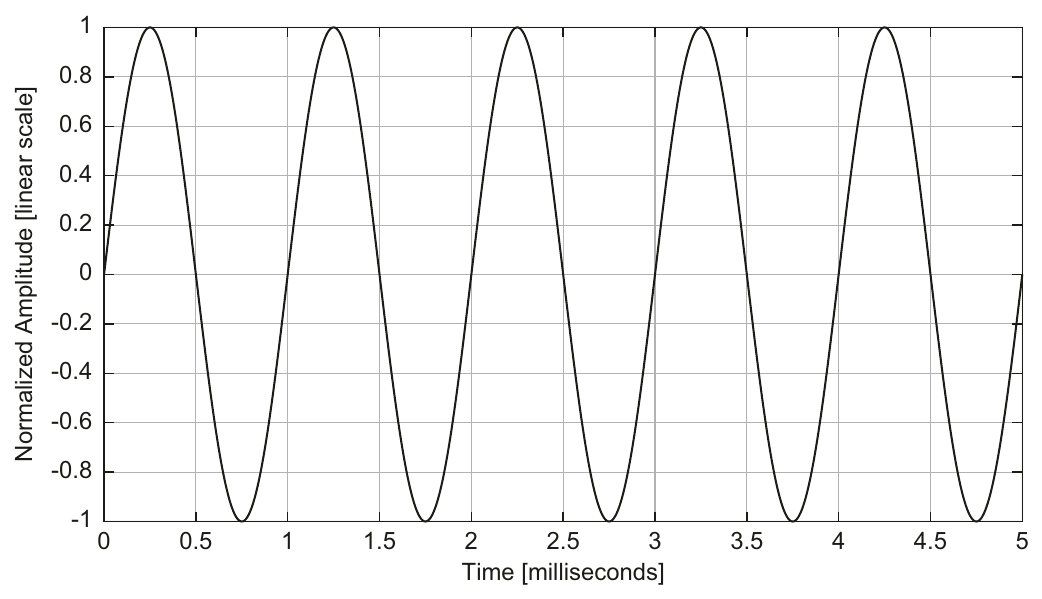
\includegraphics[width=0.7\linewidth]{img/img004}
		\caption{Sinewave 1 kHz dengan 5 siklus}
		\label{fig:img004}
	\end{figure}
\end{frame}

\begin{frame}
	\frametitle{Spektrum}
	\begin{itemize}
		\item Waveform yang periodik memiliki spektrum yang harmonik.
		\item Artinya energi hanya ada pada frekuensi yang merupakan kelipatan bilangan bulat dari frekuensi dasar/fundamental frequency ($ f_0 $).
		\item Gambar \ref{fig:img005} merupakan spektrum dari sinewave 1kHz puretone.
	\end{itemize}
\end{frame}

\begin{frame}
	\frametitle{Spektrum}
	\begin{figure}
		\centering
		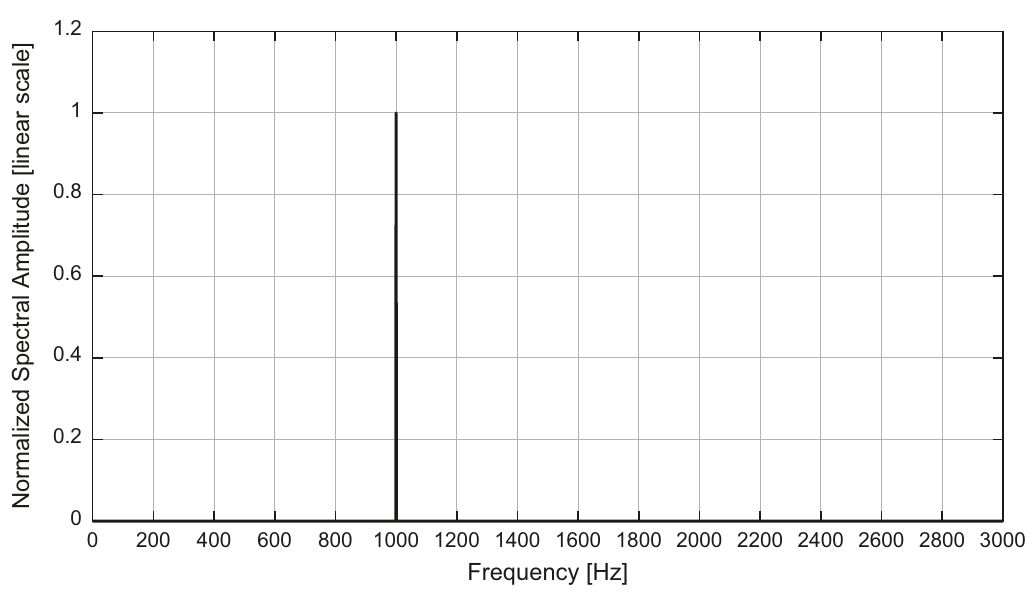
\includegraphics[width=0.7\linewidth]{img/img005}
		\caption{Magnitudo spektrum frekuensi 1 kHz puretone}
		\label{fig:img005}
	\end{figure}
\end{frame}

\begin{frame}
	\frametitle{Waveform dan Spektrum}
	\begin{itemize}
		\item Gambar \ref{fig:img006} adalah waveform periodik dan Gambar \ref{fig:img007} adalah magnitude spektrumnya.
		\item Gambar \ref{fig:img007} dapat diperoleh dengan menggunakan deret Fourier.
		\item Selain itu, transformasi Fourier dapat digunakan untuk menghitung spektrum dari waveform nonperiodik seperti yang ditunjukkan oleh Gambar dan Gambar.
		\item Nanti akan dijelaskan cara memperoleh waveform dan spektrum menggunakan Google Colab.
	\end{itemize}
\end{frame}

\begin{frame}
	\frametitle{Waveform dan Spektrum}
	\begin{multicols}{2}
		\begin{figure}
			\centering
			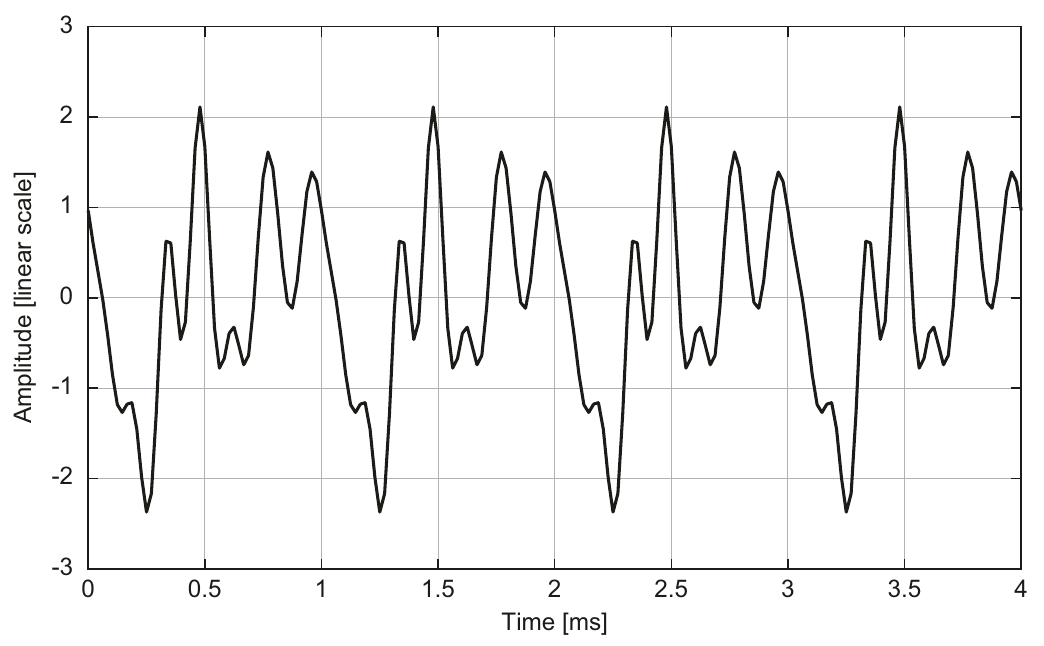
\includegraphics[width=\linewidth]{img/img006}
			\caption{Contoh waveform periodik dengan frekuensi dasar 1 kHz}
			\label{fig:img006}
		\end{figure}
		\columnbreak
		\begin{figure}
			\centering
			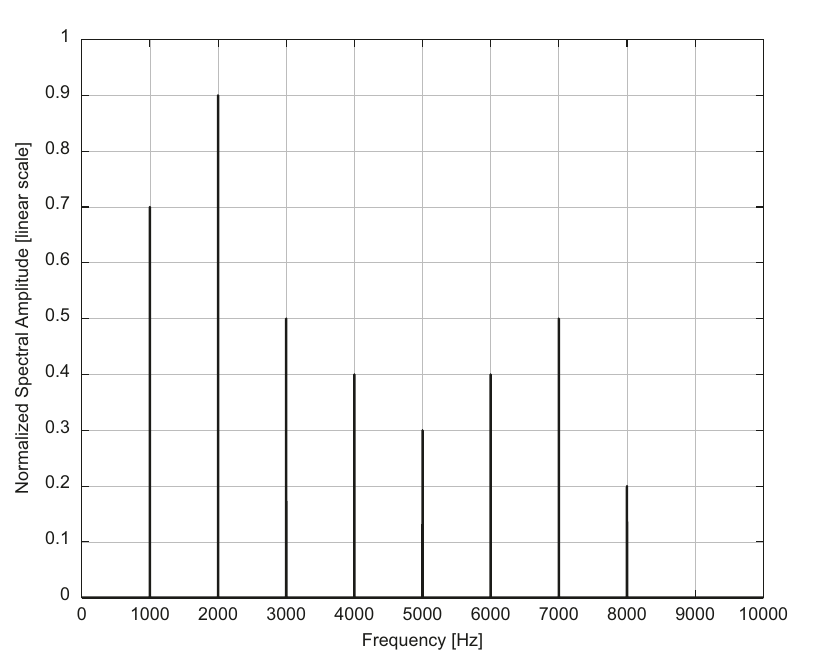
\includegraphics[width=\linewidth]{img/img007}
			\caption{Spektrum frekuensi dari waveform periodik dengan frekuensi dasar 1 kHz}
			\label{fig:img007}
		\end{figure}
	\end{multicols}
\end{frame}

\begin{frame}
	\frametitle{Spektrum dari Waveform Nonperiodik}
	\begin{multicols}{2}
		
		\columnbreak
	\end{multicols}
\end{frame}

\begin{frame}
	\frametitle{Referensi}
	\begin{enumerate}
		\item Maher, R.C., (2018). Principles of Forensic Audio Analysis. New York: Springer.
		\item https://www.gaussianwaves.com/2020/01/how-to-plot-fft-in-python-fft-of-basic-signals-sine-and-cosine-waves/
	\end{enumerate}
\end{frame}
\end{document}
